% !TEX root = main.tex
\documentclass[english,a4paper,12pt]{memoir}

\usepackage{amsmath}
\usepackage{lipsum}
\newtheorem{lemma}{Lemma}
\usepackage[draft,english]{fixme}

% ting til memoir
\setlrmarginsandblock{4.2cm}{*}{1}
\setulmarginsandblock{3.5cm}{*}{1}
\setheadfoot{2\onelineskip}{\footskip}
\checkandfixthelayout

% gør at subsections også nummeres
\setsecnumdepth{subsection}

\setcounter{tocdepth}{2}

%%%%%%
% ABSTRACT STYLE
%%%%%%
\makechapterstyle{abstract}{
  \renewcommand*{\printchaptername}{}
%  \renewcommand*{\chapnumfont}{\normalfont\sffamily\huge\bfseries}
  \renewcommand*{\printchapternum}{
    \flushleft
    \begin{tikzpicture}
      \draw[fill,color=black] (0,0) rectangle (2cm,2cm);
      \draw[color=white] (1cm,1cm) node { \chapnumfont\thechapter };
    \end{tikzpicture}
  }
 % \renewcommand*{\chaptitlefont}{\normalfont\sffamily\Huge\bfseries}
  \renewcommand*{\printchaptertitle}[1]{\center\chaptitlefont\Large##1}
}
%%%%%%

%%%%%%
% PAGESTYLE
%%%%%%
\makepagestyle{main}
\makepsmarks{main}{
  \createmark{chapter}      {both}{shownumber}{}{. \ }
  \createmark{section}      {both}{shownumber}{}{. \ }
  %\createmark{subsection}   {both}{shownumber}{}{. \ }
  % \createplainmark{toc}     {both}{\contentsname}
  % \createplainmark{lof}     {both}{\listfigurename}
  % \createplainmark{lot}     {both}{\listtablename}
  % \createplainmark{bib}     {both}{\bibname}
  % \createplainmark{index}   {both}{\indexname}
  % \createplainmark{glossary}{both}{\glossaryname}
}
\makeoddhead{main}{}{}{\rightmark}
\makeevenhead{main}{\leftmark}{}{}
% sidens fod: sidetal
\makeoddfoot{main}{}{}{\thepage}
\makeevenfoot{main}{\thepage}{}{}
% smid en linie under
\makeheadrule{main}{\textwidth}{\normalrulethickness}

% \setsecheadstyle{\large\bfseries\raggedright}
% \setsubsecheadstyle{\normalsize\bfseries\raggedright}

\nouppercaseheads
\pagestyle{main}
%%%%%%

%%%%%%
% CHAPTER PAGE STYLE
%%%%%%
% \makeoddhead{plain}{}{}{}
% \makeevenhead{plain}{}{}{}
% % sidens fod: sidetal
% \makeoddfoot{plain}{}{}{\thepage}
% \makeevenfoot{plain}{\thepage}{}{}
% \aliaspagestyle{chapter}{plain} % make chapter pages same page style as everything else


%%%%%%
% CHAPTER STYLE
%%%%%%
\usepackage[table]{xcolor}
\usepackage{tikz}

\makechapterstyle{box}{
  \renewcommand*{\printchaptername}{}
%  \renewcommand*{\chapnumfont}{\normalfont\sffamily\huge\bfseries}
  \renewcommand*{\printchapternum}{
    \flushleft
    \begin{tikzpicture}
      \draw[fill,color=black] (0,0) rectangle (2cm,2cm);
      \draw[color=white] (1cm,1cm) node { \chapnumfont\thechapter };
    \end{tikzpicture}
  }
 % \renewcommand*{\chaptitlefont}{\normalfont\sffamily\Huge\bfseries}
  \renewcommand*{\printchaptertitle}[1]{\flushleft\chaptitlefont##1}
}
%%%%%%


% used for flow charts
\usetikzlibrary{shapes,arrows}
% Define block styles
\tikzstyle{decision} = [diamond, draw, fill=blue!10,
    text width=9em, text badly centered, node distance=3cm, inner sep=0pt]
\tikzstyle{block} = [rectangle, draw, fill=blue!10,
    text width=10em, text centered, rounded corners, minimum height=4em]
\tikzstyle{line} = [draw, -latex']


\usepackage[utf8]{inputenc}	%Tillader danske tegn
\usepackage[T1]{fontenc}	%Tillader danske tegn
\usepackage{graphicx}		%Tillader indsættelse af billeder
\usepackage{dcolumn}		%Bruges til at lave matematiske tabelsøjler... se datatabel
\usepackage{mathtools}		%Ekstra matematik... bare lad den være, du får muligvis brug for den.
\usepackage{siunitx}
\usepackage{microtype}
\usepackage{amssymb}
\usepackage{rotating}

\usepackage{booktabs}
\setlength{\heavyrulewidth}{0.15em}
\setlength{\lightrulewidth}{0.08em}

% Where to look for figures
\graphicspath{ {./figures/} }

\newcommand{\mc}[1]{\multicolumn{1}{c}{#1}}
%\usepackage{threeparttable}
%\usepackage{multirow}

\numberwithin{equation}{chapter}
\numberwithin{table}{chapter}
\numberwithin{figure}{chapter}
\usepackage{varioref}
\usepackage[hidelinks]{hyperref}
\usepackage[draft]{fixme}
\linespread{1.15}
\usepackage[sc]{mathpazo}
\usepackage{wasysym}
\usepackage{cite}
\usepackage{multirow}

%\newsubfloat{figure}
%\RequirePackage[caption=false,position=top]{subfig}
%\let\subtop\subfloat

\usepackage{caption}
\captionsetup[figure]{labelfont=bf, textfont={}}
\captionsetup[table]{labelfont=bf, textfont={}}

\parindent 0pt
\setlength{\parskip}{2mm plus0mm minus0mm}

% Included chapters
\includeonly{
introduction,
theory,
simulation,
experiment,
conclusion,
appendices
}


% Macros
\newcommand{\sref}[1]{Section~\ref{#1}}
\renewcommand{\fref}[1]{Figure~\ref{#1}}
\renewcommand{\tref}[1]{Table~\ref{#1}}
\renewcommand{\eqref}[1]{Equation~(\ref{#1})}
\renewcommand{\vec}[1]{\mathbf{#1}}
\newcommand{\half}[0]{\frac{1}{2}}
\newcommand{\mean}[1]{\ensuremath{\left\langle #1 \right\rangle}}
\newcommand{\pdiff}[2]{\frac{\partial #1}{\partial #2}} % Partial derivative
\newcommand{\ppdiff}[2]{\frac{\partial^2 #1}{\partial #2^2}} % Partial derivative
\newcommand{\mat}[1]{\ensuremath{\boldsymbol{#1}}}
\newcommand{\norm}[1]{|#1|}
\newcommand{\cov}[0]{\text{cov}}
\newcommand*\chem[1]{\ensuremath{\mathrm{#1}}}

\usepackage{listings}
\usepackage{color}
\usepackage{textcomp}
\definecolor{listinggray}{gray}{0.9}
\definecolor{lbcolor}{rgb}{1,1,1}
\lstset{
	backgroundcolor=\color{lbcolor},
	tabsize=2,
	rulecolor=,
	language=matlab,
        basicstyle=\scriptsize,
        upquote=true,
        aboveskip={1.5\baselineskip},
        columns=fixed,
        showstringspaces=false,
        extendedchars=true,
        breaklines=true,
        prebreak = \raisebox{0ex}[0ex][0ex]{\ensuremath{\hookleftarrow}},
        frame=single,
        showtabs=false,
        showspaces=false,
        showstringspaces=false,
        identifierstyle=\ttfamily,
        keywordstyle=\color[rgb]{0,0,1},
        commentstyle=\color[rgb]{0.133,0.545,0.133},
        stringstyle=\color[rgb]{0.627,0.126,0.941},
}

%%%%% BEGIN DOCUMENT %%%%%
\begin{document}
\pagenumbering{roman}
\pagestyle{plain}
% !TEX root = main.tex
%% BOS FORSIDESKABELON

\begin{titlingpage}

\begin{center}

\vspace*{0cm}
\HUGE
\textsc{Hybrid Rocket Engines, Hard Starts and You}\\
\vspace{1.5cm}

%\vspace{3cm}
\makebox[\textwidth][c]{\includegraphics[width=1.2\textwidth]{frontpagerocket}}%
\vspace{1.2cm}

\large
{
    Carl-Emil Grøn Christensen\\
    Department of Physics and Astronomy, Aarhus University
}

\vspace{1.5cm}

{
  Supervisor:\\
  Gorm Bruun Andresen\\
  Department of Engineering, Aarhus University
}

\vspace{1.5cm}
{June 2016}\\


\end{center}

%\newpage

%%%%%
% The back of the frontpage
%%%%%
%colophon

\end{titlingpage}

\setcounter{page}{3}
\chapterstyle{abstract}
\vspace{6cm}
\chapter*{Abstract}
\lipsum[1-3]
\chapterstyle{box}

\newpage\thispagestyle{empty}\mbox{}\newpage
\tableofcontents*
%\newpage\thispagestyle{empty}\mbox{}\newpage
\newpage
\pagenumbering{arabic}
\setcounter{page}{1}
\pagestyle{main}

%%%%% INCLUDE CONTENT FILES %%%%%

%\include{filename}
% !TEX root = main.tex
\chapter{Introduction}

It's not rocket science.

The following report contains simulations and observations of the hybrid rocket M.E.O.W.T.H II (\textbf{M}echanical \textbf{E}ngineering \textbf{O}bservational \textbf{T}utoring \textbf{H}ybrid rocket). created by \emph{Team Rocket} at Navitas, Aarhus University. The first rocket was built in 2014 by a previous group of students, but has since been passed along to other pupils, with the intent of teaching the basics of rocket science. 


During the previous M.E.O.W.T.H.'s tests, a large pressure spike during the startup phase has been observed. This can be seen in the old video here: \url{bit.ly/1SYp1Ug} in the timespan of seconds 5-7. From the video, it appears that just as the rocket exhaust reaches supersonic speeds, \emph{something} explodes, extinguishing the flame. We know it happens before the rocket goes supersonic due to the lack of shock diamonds prior to the event.\cite[chapter 18, p.~643]{rockProp} 


This bachelor thesis attempts to simulate the rocket's startup condition in order to explain and understand the event. My advisor, Gorm Bruun Andresen, proposed a hypothesis that the pressure spike occurs at the point where mass-flow is choked in the throat. As the flow is sub-sonic, the amount of matter exiting through the nozzle is gradually increasing. When the flow goes sonic or beyond, it is suddenly capped. This abrupt change in physical properties may be able to explain this event, and the following contains the theories and thoughts that went into simulating the rocket engine's startup.


In order to create a safer rocket with more measurements options, M.E.O.W.T.H II was built. Alex Nørgaard, Gorm Bruun Andresen and I personally assembled and water-tested the rocket. The rocket can be seen on the frontpage and on figure \ref{fig:rocketpic}, and each section contains at least four possible points measurements for various instruments. 


The purpose of these simulations are ultimately to improve the rocket and rid it of large pressure variations. To see improvements, it is necessary to measure how the rocket behaves under different conditions. Therefore, setup and calibration of various measurement equipment is essential in order to retrieve excellent data. This is also covered in this report, as the experimental part is of equal importance. Measuring the rocket chamber's temperature is of great inconvenience, as the several thousands of kelvin are too much for even the strongest of thermocouples.\cite{thermocoup} This issue and it's solution is discussed thoroughly in the sections below.



All measurements and tests could not have been carried out if not for the test facilities provided by Peter Madsen of Raketmadsen's spacelaboratory. M.E.O.W.T.H II's tests were carried out on the 3rd to the 4th of May, 2016 in Copenhagen.

The entire project is publicly available on \url{https://github.com/carlegroen/bachelors_degree}, where all work files, data and various notes can be found.

% !TEX root = main.tex
\chapter{Theory}

	Understanding the theory behind the rocket's flow requires a basic knowledge of rockets. Therefore, the first theoretical segment concerns basic rocketry, followed by a more advanced segment of nozzle theory.

\section{Basic Rocket Science}

	A rocket engine consists of a few fundamental elements. A rocket engine is a type of jet engine that, in contrast to duct jets, carry their own rocket propellant. Jet engines as seen in aeroplanes are usually situated with a duct, confining the air flow. Rocket engines on the other hand carry a supply of oxygen and rocket propellant, which allows them to function even in vacuum.

	Rocket engines work by obtaining thrust in accordance with Newton's third law. The internal combustion chamber accelerates fluids through a propelling nozzle to high speeds. The fluid is most often a gas created from mixing fuel and oxidizing components in a the combustion chamber. The exhaust is accelerated to supersonic speeds by expansion in the nozzle, which forces the engine in the opposite direction.

	Most rockets used today are liquid rockets which store their propellant and oxidizing component in separate tanks. The liquid fuel is then forced into the combustion chamber for consumption. Solid-fuel rockets contain propellant prepared with a fixed fuel and oxidizing component. The fuel is called 'grain', and the storage compartment for the grain is the combustion chamber. A hybrid rocket is the mixture between the two. Most often, hybrid rockets contain a solid fuel, or 'grain' and liquid or gaseous oxygen, thus earning the name hybrid engine. Variations of this engine type do exist, but this configuration is the most often used \cite[chapter 16, p.~605]{rockProp}. Solid oxidizers are uncommon as they are problematic and have worse performance than liquid oxidizers.

	Liquid and hybrid engines both use injectors to disperse oxygen and propellant into the combustion chamber. For a hybrid engines, this means spreading oxygen to the grains surface to allow combustion.

	Hybrid rockets are inherently safer than its two counterparts, and accidents are less volatile as accidental fuel mixing is a non-issue.\footnote{Assuming you can control the oxidizer inlet valve.} The oxidizer and fuel are almost always contained in separate chambers, which also reduces the mechanical complexity of the rocket in comparison to liquid rockets.

\section{Hybrid Rocket Engine}

\begin{figure}
	\centering
	\includegraphics[width=\textwidth]{rocketsideview}
	\caption{The hybrid rocket built at Navitas in Aarhus for educational purposes.}
	\label{fig:rocketpic}
\end{figure}

	The hybrid rocket engine consists of three parts: The combustion chamber, the converging into a throat, and diverging section after called the nozzle. A rocket's effectivity is highly dependent on the shape, size and ratios between these three segments. Accordingly, it is imperative to study these parts of the rocket's design.

	The rocket in question is seen in figure \ref{fig:rocketpic} which is divided into a tank, three chambers and a nozzle. From the left: The tall tank contains the oxidizing agent, which is injected into the first part of the rocket. The oxidizing agent used is hydrogen peroxide in an $80\%$ concentration. The longest part of the rocket, as seen on figure \ref{fig:rocketpic}, contains potassium permanganate engulfed in a flame retardant foam. The mixing of potassium permanganate and hydrogen peroxide rapidly creates large amounts of oxygen, which is forced through the rocket's second part: the grain chamber. The rocket's main fuel is plain Medium-Density Fiberboard (MDF), which resides here. The energy released during decomposition heats the wooden MDF grain, until temperatures reach MDF's autoignition point of 492K at atmospheric oxygen levels \cite{mdfAIT}. Around this point the fuel combusts, and the exhaust exits through the nozzle after it has passed the mixing chamber.

	All calculations and considerations made in the report is in regard to this particular rocket. The following subsections each elaborate individual segment of the rocket, with the purpose of providing the necessary background knowledge to understand the ignition simulations and results. The explanation is given step by step, starting with injection and ending with exhaustion.


\subsection{Injection}

	To initiate combustion in the hybrid engine, an oxidizer is injected into the combustion chamber. The rocket in question creates its oxydizer by mixing an oxidizing agent with potassium permanganate. The agent is contained in a pressurized tank containing an $80 \%$ \chem{H_2O_2} rich mixture with the remainder being \chem{H_2O}. The oxidizing agent is assumed to be injected at a constant rate of:
		\begin{align}
			\dot{m}_\text{injection} = \SI{0.246}{\kg\per\s}.
		\end{align}
	in accordance to data collected at the recent launch \cite{Alex2015rapport}.

	The oxidizing agent is injected into the first chamber where decomposition into \chem{O_2} is aided by potassium permanganate. The hydrogen-peroxide (\chem{H_2O_2}) decomposes into dioxygen (\chem{O_2}) as it reacts with the potassium permanganate (\chem{K Mn O_4}), which is encased in a flame retardant foam. The balanced chemical redox reaction is as follows:
		\begin{align}
			\chem{6 KMnO_4 + H_2O_2} &\rightarrow \chem{3 K_2O_2 + 6 MnO_2 + H_2O + 3 O_2}
		\end{align}
	The specific enthalpy released during decomposition is:
		\begin{align}
			\Delta h_\text{decomposition} &= \frac{\Delta H_\chem{H_2O_2}}{\text{M}_\chem{H_2O_2}}
		\end{align}
	Where $\Delta H$ is the change in enthalpy. The energy released heats the grain's surface to autoignition temperatures of approximately $\SI{220}{\celsius}$ in this extremely oxygen-rich environment. The increased temperature increases the pressure, in accordance to the ideal-gas law:
		\begin{align}
			P V &= n R T
		\end{align}
	Which is assumed to be valid as the gas is approximately stagnant in the mixing chamber \cite{atkins}.
	The ideal gas law is crucial in our description of the rocket. Describing the rocket's upstart phase requires coupling the changes in temperature $T$, pressure $P$ and amount of substance $n$. During injection and decomposition, combustion occurs simultaneously.

	\subsection{Combustion Chamber}

		The combustion chamber contains two important theoretical aspects. First, the propellant grain has significant effects on the rocket's thrust over time. Secondly, the theoretical description of the rocket's combustion allows us to estimate different working parameters, and deciding the rocket nozzle's size and area ratios.

	\subsubsection{Propellant Grain}

		The combustion chamber consists of an approximate 3 liter cavity which is filled with the grain. The actual volume in a hybrid rocket depends strongly on the initial condition of the grain and the fuel's combustion rate. Holes have to be carved in the grain to allow oxygen to reach the grain's surface, and transport exhaust towards the throat. The combustion rate is largely determined by the exposed surface area of the grain, and the flux of the oxidizer. The surface gradually expands as the outer regions are burned away, thus changing the rocket's effective thrust over time \cite[chapter 12, p.~174]{ignition}. The propellant's increase in burning area during ignition is assumed to be negligible, compared to the rapid increases in pressure and temperature.

				\begin{figure}
					\centering
					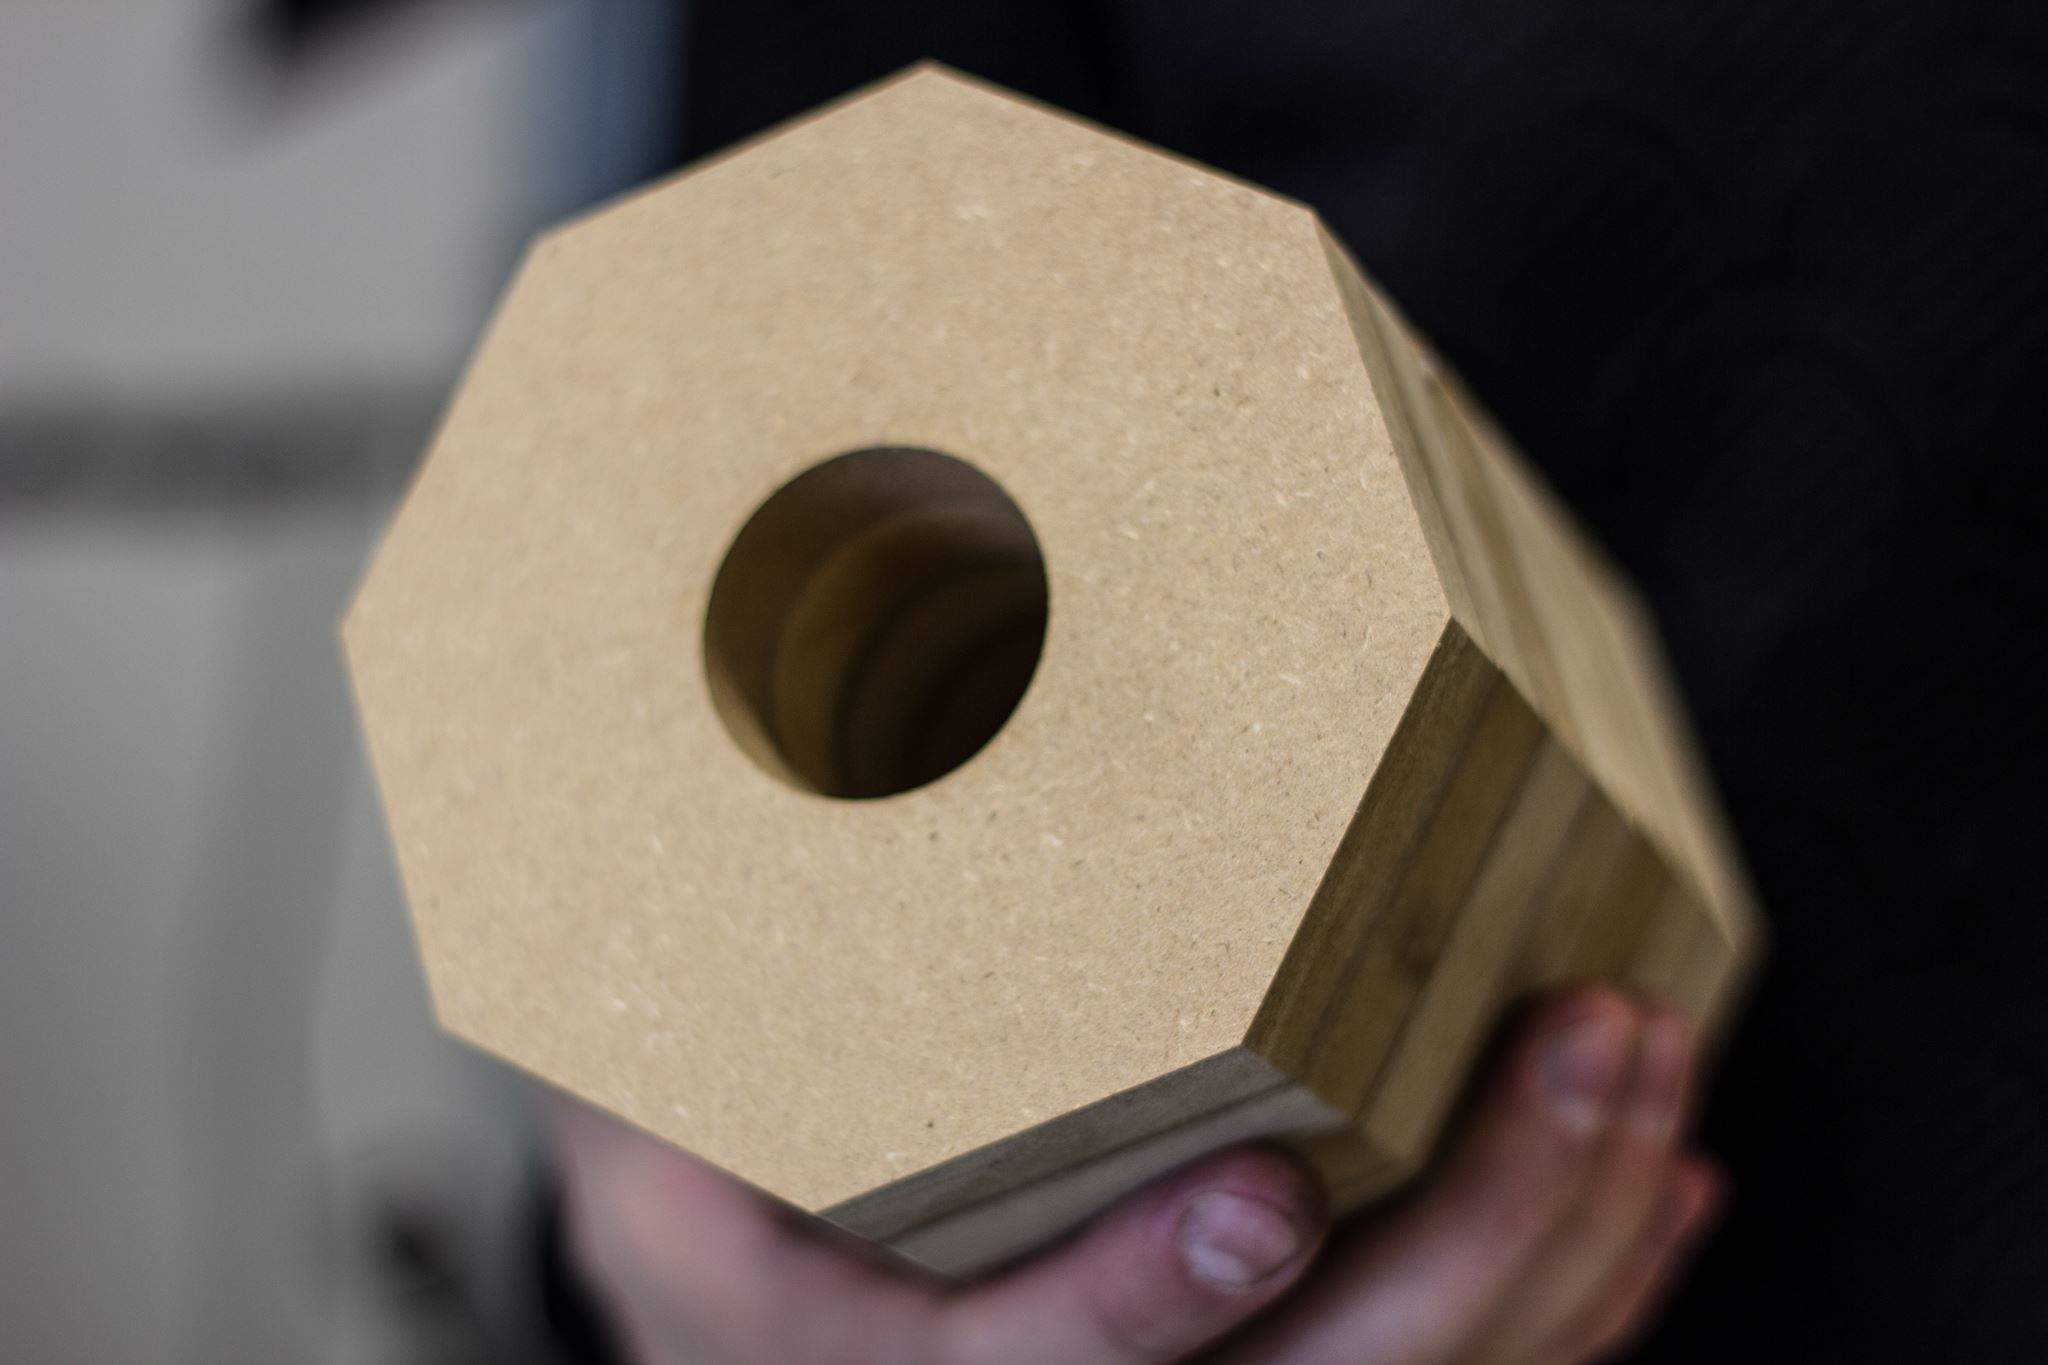
\includegraphics[width=\textwidth]{singlehole}
					\caption{Example of MDF grain with a single combustion--hole. This will have a uniformly increasing regression-rate, as the burning area increases evenly.}
					\label{fig:singlehole}
				\end{figure}

		The shapes and sizes of the holes in the grain has a large impact on the initial ignition and thrust ratios \cite{nakka}. An example of a single hole configuration can be seen in figure \ref{fig:singlehole}, and more examples can be found on \url{http://www.nakka-rocketry.net/th_grain.html}, along with a general performance description. Depending on the surface areas and designs, the different grain's regression rate varies greatly over time. The regression rate will be proportional to the thrust, unless oxygen is the limiting factor. The generated thrust is directly proportional to the instantaneous burning area, and as this area increases, so does the thrust.

			\begin{figure}
				\centering
				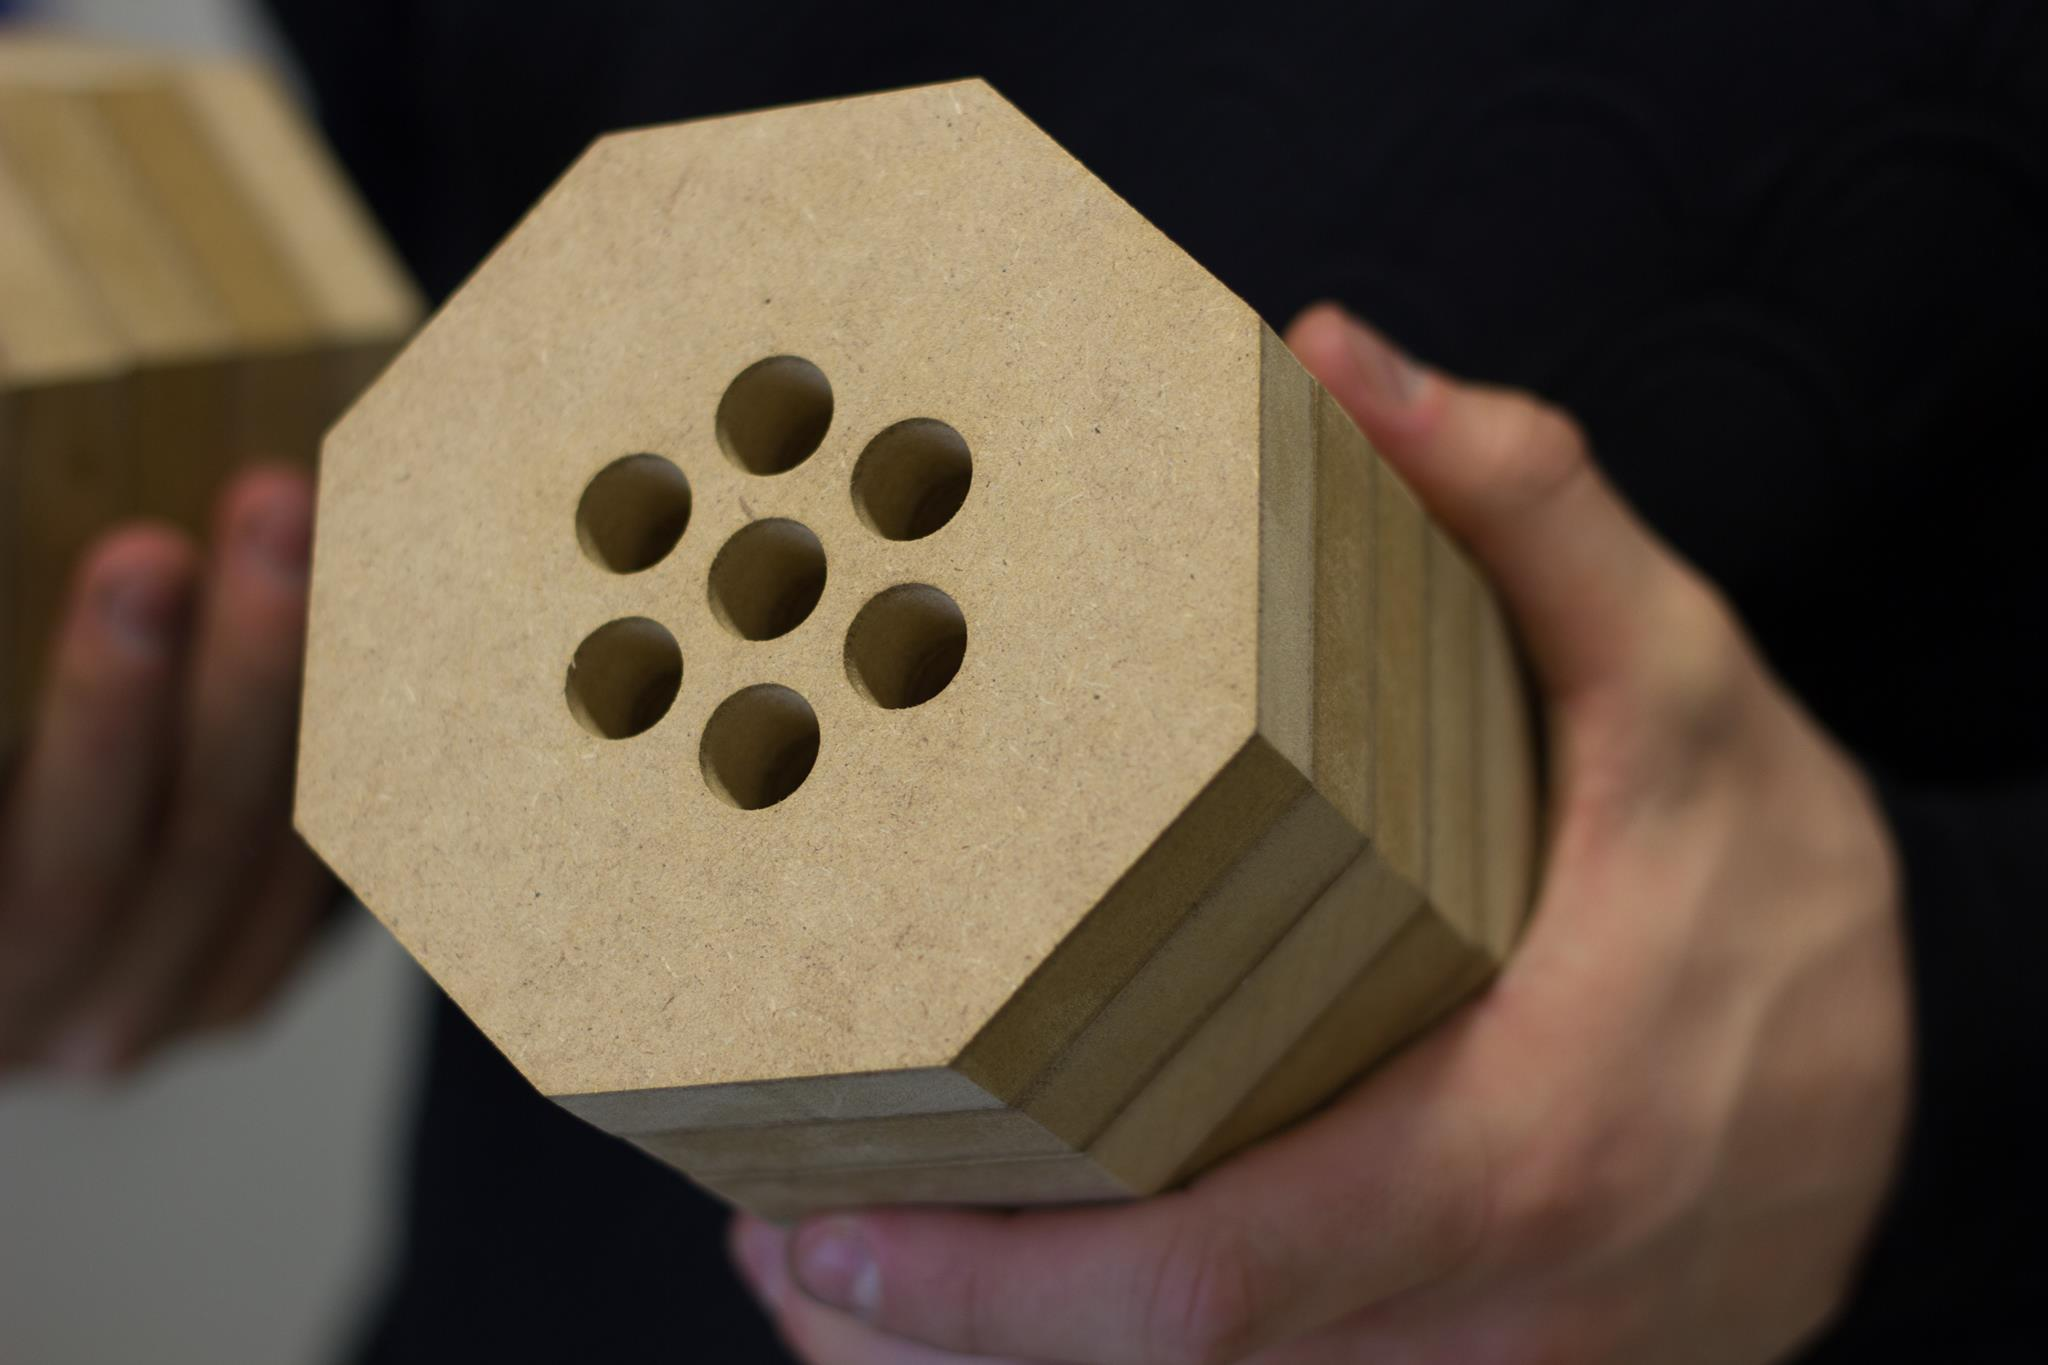
\includegraphics[width=\textwidth]{wagonwheel}
				\caption{The wagon-wheel design used in all rocket tests concluded in this report. The large surface area allows combustion on a larger surface, which gives more effective combustion.}
				\label{fig:wagonwheel}
			\end{figure}

		An alternative explanation to the pressure spike could therefore be a very fast increase in regression area. The grain's specifications from the previous tests are not mentioned, but a wagon--wheel design as seen in figure \ref{fig:wagonwheel} with several holes could allow ignition in single canals before all of them. This could allow hot pyrolytic fuel and oxygen to accumulate, causing an eventual explosion. The large surface area of the wagon--wheel design is allows for cleaner, more efficient combustion, and it is therefore the preferred setup for our experiments \cite{nakka}.

	\subsubsection{Autoignition}

		There are two types of ignition: Autoignition and piloted ignition \cite[chapter 4, pp.~66]{principlesoffire}. Piloted ignition is the process of flame propagation in a premixed fuel system, such as lighting a candle or starting a petrol engine. This is the usual way of igniting every day systems, however, MEOWTH uses the other type: Autoignition.

		Autoignition occurs without a spark of flame present. The fuel must have a certain concentration and temperature, before spontaneously igniting. This temperature is lowered by rising oxygen concentration and pressure, which complicates setting a specific point of time of ignition \cite{ASTMautoign}. According the the MDF's datasheet \cite{mdfAIT}, autoignition occurs around \SIrange{220}{250}{\celsius}. This minimum temperature tells us when spontaneous combustion takes place, the question is then how quickly after reaching this temperature does the material ignite?

		Autoignition time $t_\text{auto}$ for thick materials (thicker than $\SI{2}{mm}$) is given by:
		\begin{align*}
			t_\text{auto} &= C (k \rho c) \left[\frac{T_\text{auto} - T_\text{initial}}{\phi} \right]^2
		\end{align*}
		where $k$ is the thermal conductivity of the material, $C$ is a constant depending on the heat flux, but roughly equivalent to $0.785$ assuming no heat loss \cite[chapter 4, pp.~71]{principlesoffire}. $T_\text{auto}$ is the autoignition temperature and $T_\text{initial}$ is the starting temperature, and $\phi$ is the heat flux.

		Back--of--the--envelope calculations shows that the autoignition time is on the order of magnitude $10^{-5}$, which is way faster than anything we should be able to measure. The temperature and pressure rise far too quickly for this to have an obvious effect on the ignition. It is thus assumed to be far too small to have any real influence, compared to the autoignition temperature.

	\subsubsection{Combustion}

		As temperatures reach the MDF's autoignition point, and oxygen levels increase, combustion starts taking place. The combustion reaction can be described chemically by the formula:
			\begin{align}
				\chem{C_3 H_4 O_2 + 3 O_2} &\rightarrow \chem{3 CO_2 + 2H_2O}
			\end{align}
		Energy released in this reaction heats up the chamber's fluids towards a design temperature of $\SI{2498}{K}$. Assuming a \emph{closed} chamber, the rise in temperature and amount of substance yields a rapid increase in pressure over time. This is not a desired property, as that would eventually lead to engine destruction. The accumulated decomposed and combusted material leaves through the rocket's throat, which allows the rocket to reach pressure-equilibrium. The throat's area is essential to the rocket's pressure and thus stability, hence the advance to the throat.

\subsection{Throat}

	\begin{figure}
		\includegraphics[width=\textwidth]{elon3}
		\caption{Cross section of the throat area.}
		\label{fig:crossthroat}
	\end{figure}

	The throat begins at the end of the combustion chamber, at the opposite side of where injection occurs. The throat is characterized by the convergence of the rocket chamber into a small passage called the throat, followed by a diverging section: The nozzle. The throat's cross-sectional area is what determines the maximum flow rate, as the speed of sound restricts the flow of matter. In order to calculate the amount of matter contained in the chamber, it is crucial to know how much is flowing out. Due to conservation of mass, the flow rate $\dot{m}_t$ must be proportional to the density of the material, the velocity and the throat's area according to \cite{nasacompflow}:
		\begin{align}
			\dot{m}_t &= \rho \cdot v_t \cdot A_t
		\end{align}
		The velocity $v_t$ is thus roughly proportional to the mass flow as the area and density are approximately constant in this case. Hence, as the matter approaches the speed of sound, the flow rate out of the rocket stagnates. This is called mass flow choking, which must be at a maximum when the velocity is equal to the speed of sound. This condition is satisfied when the mach number $M=1$. For an ideal compressible gas, this becomes:
		\begin{align}
			\dot{m}_t &= \frac{A_t P_c}{\sqrt{T_t}} \sqrt{\frac{\gamma}{\text{R}}} \left(\frac{\gamma+1}{2}\right)^{-\frac{\gamma+1}{2(\gamma-1})}
		\end{align}
	Where $P_c$ is the pressure in the combustion chamber, $T_t$ is the temperature in the throat, $\gamma$ is the specific heat ratio and R is the gas constant \cite{nasacompflow}. Three outcomes are possible:
	\begin{align*}
		\dot{m}_t < \dot{m}_{in} & ~,~ \text{less mass is coming out than is flowing "into" the rocket.} \\
		\dot{m}_t = \dot{m}_{in} & ~,~ \text{mass outflow equilibrium.} \\
		\dot{m}_t > \dot{m}_{in} & ~,~ \text{more mass is flowing out than is being created.}
	\end{align*}
	The first outcome would yield increasing pressure until the rocket has burned all of it's fuel, or it explodes. The second option is what we know as a safe and steady rocket, assuming the designed mass flow equilibrium is within the rocket's boundaries. The final outcome will yield a slow decrease in pressure over time, until the rocket has been exhausted for material inside and combustion ceases. \fxnote{Passer det med masse?}

	In order to describe the initial pressure spike it is necessary to not assume any of these conditions. The abrupt change from the first to the second condition was initially hypothesized to cause the spike in pressure. Therefore, simulating the mass flow out of the rocket is essential to our understanding of the phenomenon. This does however require knowledge of several key parameters within the rocket, which are difficult to calculate, unless some things are assumed, such as conservation of entropy. However, in order to combine this knowledge, we first have to look at the final piece.

\subsection{Nozzle}

	\begin{figure}
		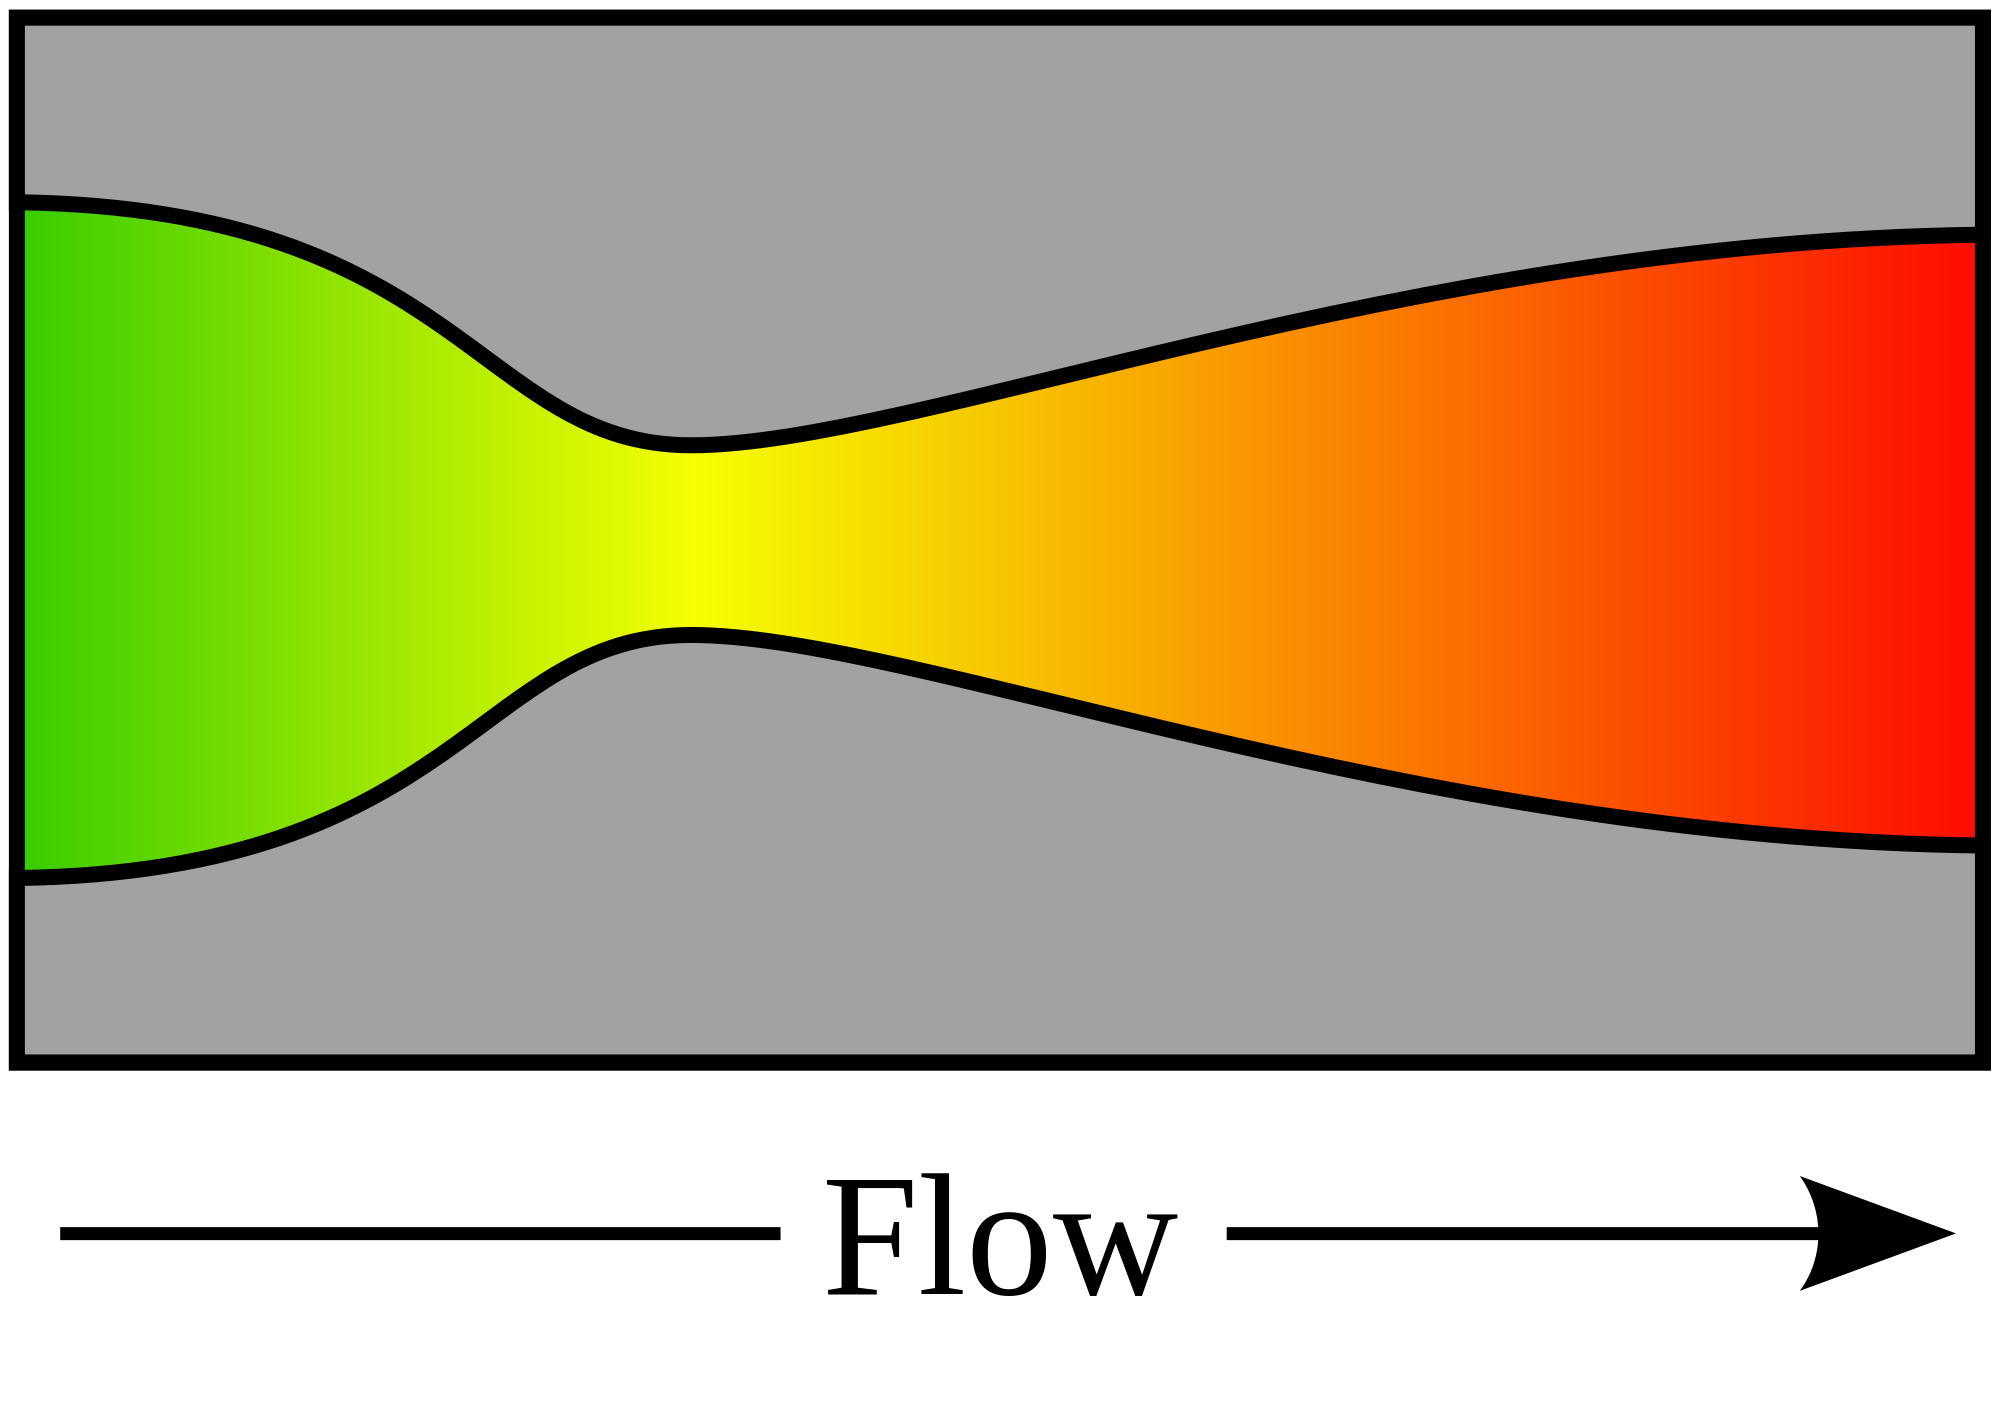
\includegraphics[width=\textwidth]{delaval}
		\caption{Schematic of a de Laval nozzle, where the green area is equivalent to the mixing chamber, and the red area is the nozzle's exit.}
		\label{fig:delaval}
	\end{figure}

	The rocket nozzle's primary function is to channel the combusted propellant out of the rocket and accelerate it. The optimal nozzle maximizes the velocity of the exhaust, preferably to supersonic values. The most well-known nozzle is a convergent-divergent nozzle called a deLaval Nozzle, which performs all of these things through simple geometry. Such a nozzle can be seen on figure \ref{fig:delaval}, where the combustion chamber is to the left, and the exhaust is to the right. An important part of maximizing the nozzle's performance is ensuring that the flow stays isentropic. At optimal ratios, the flow is frictionless and adiabatic, which ensures entropy is conserved. Isentropic flow is considered to \emph{only} be dependent on the cross-sectional area of the nozzle that the fluid moves through \cite{nakkanozz}.

	As the fluid is pushed through the throat it is highly pressurized. The nozzle is in contact with the surroundings, which acts as a reservoir of low-pressure gas between atmospheric pressure ($\SI{101.3}{kPa}$).
	and no pressure (in space!), depending on the rocket's whereabouts. The expansion of course depends on the surrounding pressure, but in general, the plume can be over- and underexpanded and ambient. Ambient is the preferred expansion of the plume, where the exhaust gas is in pressure equilibrium with the surrounding air. If the exhaust has the same pressure as the surroundings, the gas is optimally expanded, and provides the maximum amount of thrust to the rocket \cite{robertnozzle}.

\section{Heat Capacity}

 \begin{align}
	 \gamma &= \frac{C_p}{C_v}
 \end{align}

\section{Isentropic Flow}

	In order to effectively describe the rocket's behavior, we have to assume a few things:
	\begin{enumerate}[topsep=0pt,itemsep=-1ex,partopsep=1ex,parsep=1ex]
		\item{Entropy is conserved.}
		\item{Decomposition and combustion products obey the perfect gas law.}
		\item{All chemical reactions are adiabatic: No heat is lost to the surroundings.}
		\item{The fluid velocity inside the chamber is approximately zero, allowing us to assume stagnated pressure. The velocity is \emph{not} assumed to be zero when entering the throat and nozzle, however.}
	\end{enumerate}

	The assumption of isentropic flow stems from the idea that the process is reversible. The fluid will, after moving through the nozzle, have the same original values. The second law of thermodynamics states that reversible flow maintains entropy, and this allows us to calculate almost any value related to the rocket's flow. It is therefore an essential piece to the project \cite{nakkanozz}.

	If supersonic flow is not achieved by gradual means, isentropic flow is not a valid assumption. If shock waves occur abruptly, isentropic flow is not a valid assumption. Hence, exit values are simulated before any normal or oblique shock relations occur \cite{nasaisentrop}.

	The simulation is based on four valuable equations: The conservation of energy, the continuity equation, the momentum equation and equation of state.

	\begin{figure}
		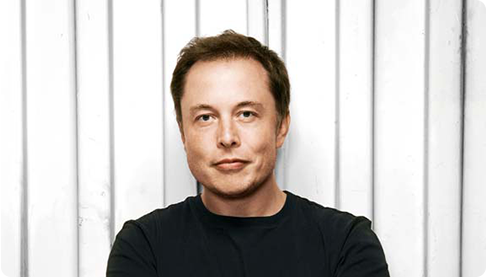
\includegraphics[width=\textwidth]{elon2}
		\caption{Isentropic flow between two points $x_1$ and $x_2$ in the rocket.}
		\label{fig:isentropicflow}
	\end{figure}


	Conservation of energy requires that for adiabatic flow, between two any points $x_1$ and $x_2$, as seen in figure \ref{fig:isentropicflow}:
	\begin{align}
		h_1 - h_2 & = \frac{1}{2} (v_2^2 - v_1^2) = C_p (T_1 - T_2)
		\intertext{where $h$ again is the enthalpy of the fluid, $v$ is the flow velocity and $C_p$ is the heat capacity, T is the fluid's temperature. From the continuity equation, we can find a pseudo-steady state from looking at the stagnation temperature in the chamber. Setting $v_2 = 0$ yields the stagnation temperature:}
		T_0 &= T + \frac{v^2}{2 C_p}
		\intertext{This yields several key relationships between stagnation properties for pressure, density and temperature:}
		\frac{T_0}{T} & = \frac{P_0}{P}^{\frac{\gamma-1}{\gamma}} = \frac{\rho_0}{\rho}^{\gamma-1}
		\intertext{\cite[chapter 3, p.~60-63]{turbomac} Using this, we can find the temperature at the exit:}
		T_e &= \frac{P_e}{P_0}^{1-\frac{1}{\gamma}} \cdot T_0
		\intertext{As $P_e$ is the exit pressure, which is equivalent to the ambient pressure. The exit temperature allows us to calculate the density of the exiting fluid $\rho_e$:}
		P_e &= \rho_e R T_e \Rightarrow \rho_e = \frac{P_e}{R T_e}
		\intertext{Bernoulli's equation provides us with the exit velocity $v_e$:}
		v_e &= \sqrt{2 \frac{P_0-P_e}{\rho_e}} = \sqrt{2 \frac{P_0-P_e}{\frac{P_e}{R T_e}}}\\
		&\Rightarrow  \sqrt{2 \frac{(P_0-P_e)R T_e}{P_e}}
		\intertext{Exit velocity and density yields the mass outflow per second:}
		\dot{m}_\text{out} &= A_e \cdot v_e \cdot \rho_e
		\intertext{and knowing how much matter is flowing "into" the rocket (see injection and combustion chamber sections) yields the total enthalpy contained in the rocket at all times. Therefore, we can now approximate the temperature in the rocket's chamber, knowing the different material's abundances.}
	\end{align}

% !TEX root = main.tex
%%%% Colour Palette %%%%%
\definecolor{black1}{RGB}{0,0,0}
\definecolor{orange1}{RGB}{230,159,0}
\definecolor{skyblue}{RGB}{86,180,233}
\definecolor{blueishgreen}{RGB}{0,158,115}
\definecolor{yellow}{RGB}{240,228,66}
\definecolor{blue1}{RGB}{0,114,178}
\definecolor{vermillion}{RGB}{213,94,0}
\definecolor{reddishpurple}{RGB}{204,121,167}
%%%%%% Block Styles %%%%%%%%%%%%%%%%%%%%%%%%%%%%
\tikzstyle{decision} = [diamond, draw, fill=blueishgreen,
    text width=4.5em, text badly centered, node distance=3cm, inner sep=0pt]
\tikzstyle{block} = [rectangle, draw, fill=skyblue,
    text width=5em, text centered, rounded corners, minimum height=4em]
\tikzstyle{line} = [draw, -latex']
\tikzstyle{cloud} = [draw, ellipse,fill=yellow, text width=5.5em, node distance=3.5cm,
    minimum height=2em]
%%%%%%%%%%%%%%%%%%%%%%%%%%%%%%%%%%%%%%%%%%%%%



\chapter{Simulation}\label{cha:simulations}

  Using the previous theory, simulating the rocket's ignition phase can be done using only a fairly small sample of data. Molar masses, gas constants and the like are all table constants. Given ambient pressure $P_0$, temperature $T_0$ and chamber volume $V_\text{chamber}$, initial conditions can be calculated. As the rocket takes off, using the mass flow $\dot{m}$ and fraction of oxygen being consumed in combustion $f$, we can compute the rocket's performance at all times assuming isentropic flow. The inner pressure and temperature can be found by calculating the flow into and out of the rocket, as well as the energy released in the various chemical reactions.
%
\begin{figure}
	\centering
	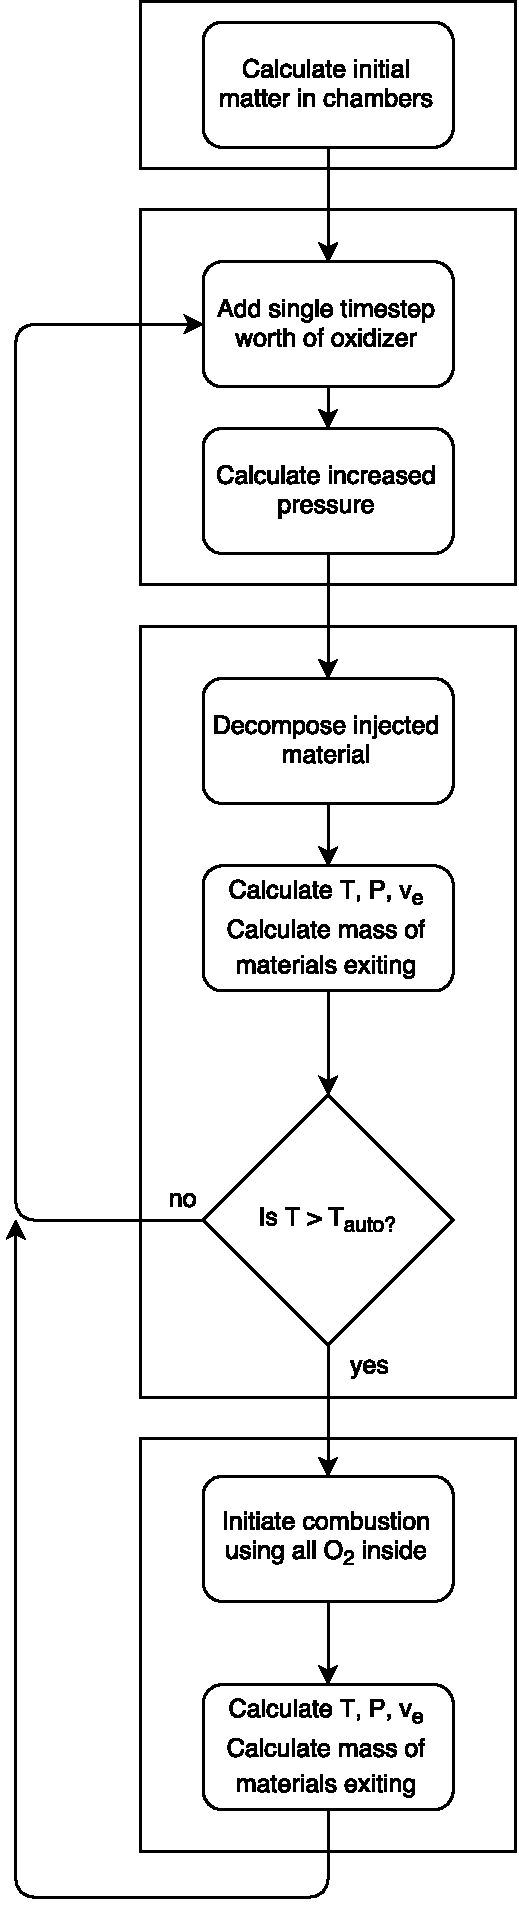
\includegraphics[width=0.45\textwidth]{rocketflowchart.pdf}
	\caption{Scheme showing the implementation of the rocket's ignition algorithm.}
	\label{fig:flowchart}
\end{figure}


\section{Implementation}

  The rocket engine's ignition algorithm is based on the previous assumptions. Figure \ref{fig:flowchart} shows a flowchart of the ignition algorithm. The implemented algorithm is divided into four parts, which determine the rocket's performance at various stages. The first stage is the rocket's pre--launch conditions, eg. amount of substance $n$, pressure $P$ and temperature $T$. The second stage is injection of oxidizer into the pre--combustion (or decomposition) chamber. The amount of injected oxidizer is equivalent to the injection nozzle's flow per time step $\Delta t$ in every iteration. This is followed by recalculating the rocket's conditions. After the initial matter has been injected, decomposition starts. This is the third stage of the algorithm. Post decomposition, the temperature, pressure, exit velocity $v_e$ and exit mass can be found. The temperature is compared to the autoignition temperature $T_\text{auto}$: If higher, combustion of material still contained inside the rocket starts. Otherwise, more oxidizer is injected and decomposed until the energy released during decomposition heats the interior to autoignition temperatures. The final stage occurs when temperatures are large enough to allow combustion. Combustion expends \emph{all} the available oxygen inside the rocket during every iteration. This means, that if $T_\text{auto} \approx T_\text{amb}$, combustion occurs instantaneously, using only the oxygen released by the first time step's oxidizer. If, however, $T_\text{auto} > T_\text{amb}$ (as it is in our case), combustion occurs a certain time later, allowing oxygen to accumulate inside the chamber.
  
  The code runs until the simulation software eventually crashes, as that is sadly the bottleneck of the operation. The simulation is done in part by MatLAB and part by Engineering Equation Solver (EES). EES is rather un--robust and crashes after a number of iterations, why is not exactly certain. This also explains why the simulations stop in the following section, before all of them reach their steady--state perfectly.

\section{Results}

  \begin{figure}
  	\centering
  	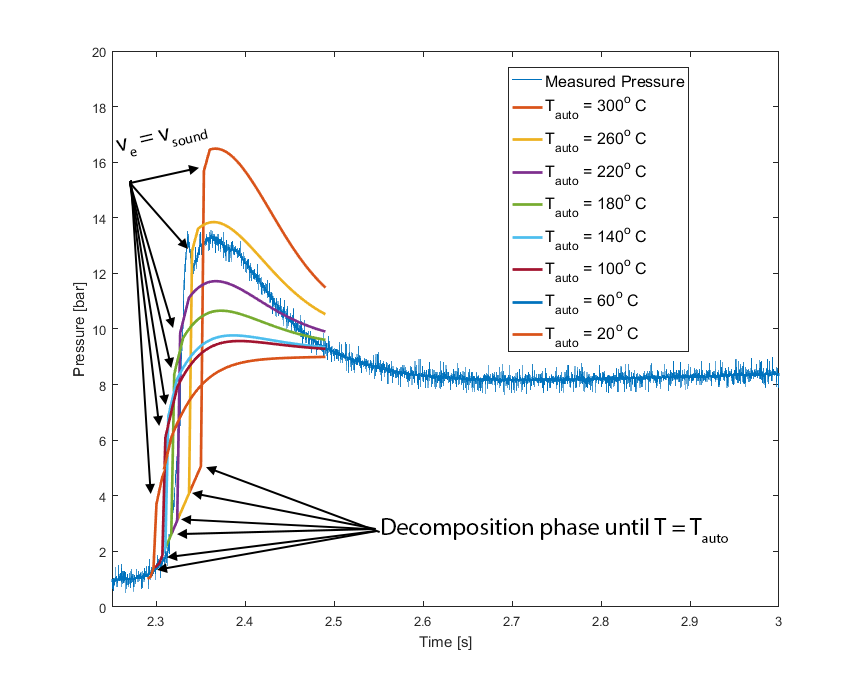
\includegraphics[width=\textwidth]{pressureovertime3}
  	\caption{Pressure over time for different autoignition temperatures $T_\text{auto}$. The highest peak is given by the highest autoignition temperature. The first linear phase at the bottom is where decomposition happens without combustion. When the curve breaks, combustion occurs. Instantaneously after combustion, all models' exit velocities reach the speed of sound.}
  	\label{fig:pressureovertime}
  \end{figure}

  The simulation shows promising results in the description of the hybrid engine's pressure spikes. In figure \ref{fig:pressureovertime} the simulations are plotted on top of the second test experiment in order to give a feeling of the peak sizes. The simulations start with an increase in pressure moving sporadically, due to phase--shifts in the propellants, oxidizing agent and air contained inside. As decomposition starts, pressure increases linearly until autoignition temperatures are reached, and a sudden spike in pressure appears. 
  
  As it appears from figure \ref{fig:pressureovertime}, the higher the autoignition temperature the higher the peak pressure is. Thereto, the higher the peak, the later combustion takes place. This is to be expected, as a higher autoignition point allows more oxygen to accumulate in the chamber which of course takes more time. All of the simulations tend toward a steady-state at the end, where they would eventually meet at the design--pressure. The yellow, low auto-ignition point of $\SI{60}{\celsius}$ steadily and cleanly tend toward the design--pressure, as would be preferred for the hybrid rocket. The steady increase ensures no rapid combustion happens, and transitions between the ignition states flow without problem. This result proposes the hypothesis, that a reduction of the autoignition temperature, or the presence of a pilot flame might be able to extinguish the unwanted spiking behavior.
  
  

  \begin{figure}
  	\centering
  	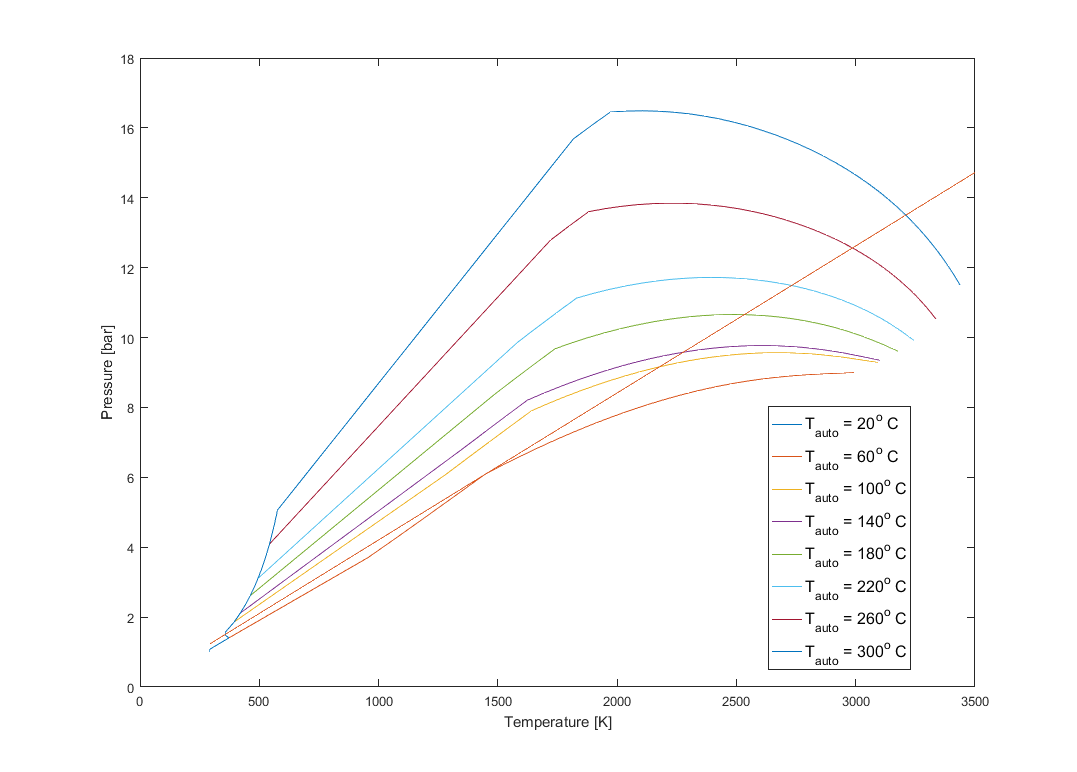
\includegraphics[width=\textwidth]{pressurepertemperature}
  	\caption{Pressure per temperature for different autoignition temperatures $T_\text{auto}$. The straight line is a theoretical fit assuming constant amount of substance $n$.}
  	\label{fig:pressurepertemperature}
  \end{figure}

  In figure \ref{fig:pressurepertemperature} we see the pressure plotted against temperature in the simulation, with a linear theoretical fit of the rocket's design values. After initial spiking, the graph "necks" due to the rocket reaching maximum the speed of sound. The pressure drops as the temperature increases up to very large values of almost $\SI{3500}{\kelvin}$. The pressure should stabilize steadily towards the end, but all simulations show a trend of pressure dropping with increasing pressure. However, the rocket is designed to work at a temperature of $\SI{2500}{\kelvin}$, and the pressure values around this area varies between $\SI{8.8}{\bar}$ and $\SI{16.2}{\bar}$ -- somewhat within the design pressure of $\SI{10}{\bar}$.

  %
  % \section{Stage one: Injection}
  %
  %
  %
  % \section{Stage two: Decomposition}
  % \section{Stage three: Combustion}
  % \section{Stage four: Thrust}
  %
  %
  % \begin{tikzpicture}[node distance = 3cm, auto]
  %     % Place nodes
  %     \node [block] (const) {Define constants};
  %       \node [cloud, left of=const] (constvars) {$T_{amb}$, chamber dim., etc.};
  %     \node [block, below of=const] (inj) {Define injection rates per second};
  %       \node [cloud, left of=inj] (injvars) {$\dot{n}_{H_2O_2,1}$ $\dot{n}_{H_2O,1}$};
  %     \node [block, below of=inj] (dec) {Define decomposition rates per second};
  %       \node [cloud, left of=dec] (decvars) {$\dot{n}_{H_2O_2,2}$ $\dot{n}_{H_2O,2}$ $\dot{n}_{O_2,2}$};
  %     \node [block, below of=dec] (com) {Define combustion rates per second};
  %       \node [cloud, left of=com] (comvars) {$\dot{n}_{H_2O,3}$ $\dot{n}_{O_2,3}$ $\dot{n}_{CO_2,3}$};
  %     \node [block, below of=com] (exha) {Define exhaustion mass flow};
  %       \node [cloud, left of=exha] (exhavars) {$\dot{m}_{pla,3}$};
  % %%%% Defining more relavant stuff %%%%%
  %     \node [block, below of=exha] (mflow) {Define mass flow rates $n$ per time step $dt$ to find enthalpy};
  %       \node [cloud, left of=mflow] (mflowvars) {$m_{tot,n} = \sum\limits_{\text{chem.} 1}^{\text{chem. k}} \dot{n}_j \cdot dt$};
  %     \node [block, right of=mflow] (mfrac) {Calculate mass fraction in flow rates to calculate enthalpy leaving rocket later};
  %     \node [block, above of=mfrac, node distance=6cm] (refent) {Calculate reference enthalpy in decomposition and combustion states};
  %       \node [cloud, right of=refent] (refentvars) {$H = \sum \dot{m}_{j} \cdot H_j(P,T) + \Delta h_{dec,com} \cdot \dot{m}_\chem{H_2O_2} \cdot dt$};
  %     \node [decision, right of=const, node distance=5cm] (next) {Passes static data into $P$ and $T$ calculations};
  %
  %
  %     % Draw edges
  %     \path [line] (const) -- (inj);
  %     \path [draw] (const) -- (constvars);
  %     \path [line] (inj) -- (dec);
  %     \path [draw] (inj) -- (injvars);
  %     \path [line] (dec) -- (com);
  %     \path [draw] (dec) -- (decvars);
  %     \path [line] (com) -- (exha);
  %     \path [draw] (com) -- (comvars);
  %     \path [draw] (exha) -- (exhavars);
  %     \path [line] (exha) -- (mflow);
  %     \path [draw] (mflow) -- (mflowvars);
  %     \path [line] (mflow) -- (mfrac);
  %     \path [line] (mfrac) -- (refent);
  %     \path [draw] (refent) -- (refentvars);
  %     \path [line] (refent) -- (next);
  % \end{tikzpicture}
  %
  % INSERT FLOWCHART OF SECONDARY PART WHEN POWERPOINT WORKS



% \begin{tikzpicture}[node distance = 2cm, auto]
%     % Place nodes
%     \node [block] (init) {initialize model};
%     \node [cloud, left of=init] (expert) {expert};
%     \node [cloud, right of=init] (system) {system};
%     \node [block, below of=init] (identify) {identify candidate models};
%     \node [block, below of=identify] (evaluate) {evaluate candidate models};
%     \node [block, left of=evaluate, node distance=3cm] (update) {update model};
%     \node [decision, below of=evaluate] (decide) {is best candidate better?};
%     \node [block, below of=decide, node distance=3cm] (stop) {stop};
%     % Draw edges
%     \path [line] (init) -- (identify);
%     \path [line] (identify) -- (evaluate);
%     \path [line] (evaluate) -- (decide);
%     \path [line] (decide) -| node [near start] {yes} (update);
%     \path [line] (update) |- (identify);
%     \path [line] (decide) -- node {no}(stop);
%     \path [line,dashed] (expert) -- (init);
%     \path [line,dashed] (system) -- (init);
%     \path [line,dashed] (system) |- (evaluate);
% \end{tikzpicture}

% !TEX root = main.tex
\chapter{Rocket Tests}\label{cha:experimental}

	MEOWTH II was tested at Peter Madsen's space laboratory in Copenhagen, on the 3rd to the 4th of May 2016 by Team Rocket of Navitas. The whole ordeal has spawned several articles, which the interested reader can find in appendix \ref{App:A}. A  complete logbook along with a firing procedure can be found in appendix \ref{App:B}.

	The test setup can be seen in figure \ref{fig:rocketpic}, and the first burn can be seen on the front page. The test stand consists of a metal fixture that holds the rocket in a horizontal position, with the hydrogen--peroxide tank standing vertically. The metal fixture keeps the rocket from moving under tests. Sandbags are placed on top in order to stop fast--moving shrapnel, in case of a complete engine destruction. Further safety instructions can also be found in appendix \ref{App:B}.

	The purpose of the experiments was to measure the variations in pressure throughout the rocket. The following will be an analysis of the data collected, along with a brief description of the sensors involved. A group consisting of three students also took video footage of the tests in order to analyze the rocket's shock diamonds, this will not be treated here, however.

	\section{Equipment}

	Eight pressure sensors were mounted on the rocket, ranging over three measurement frequencies: $\SI{250}{\Hz}$, $\SI{2000}{\Hz}$ and $\SI{20000}{\Hz}$. All were measured at $\SI{20000}{\Hz}$, which means the slower sensors are oversampled. One of each sensor was placed in both the rocket's mixing chamber and decomposition chamber. The two remaining sensors, a slow and a fast, were mounted by the hydrogen--peroxide tank. The measurement equipment was connected to a DAta Acquisition (DAQ) system from National Instruments, which in turn was connected to the data--logging software LabVIEW on a nearby slave unit. The slave unit was remotely controlled by a computer inside the safety--submarine, which allowed ignition and data--logging nearby the test site without being in danger.

	Two manometers were placed before and after the pressurization valve, in order to manually check the tank's pressure before ignition.

	A more thorough discussion of project improvements can be found in chapter \ref{cha:perspective}. A more thorough discussion of individual sensors and specific sensor result can be found in my brother--groups report here: \url{https://github.com/carlegroen/bachelors_degree/tree/master/cousinprojects/}.

	\section{Experimental Procedure}

	\begin{figure}
		\centering
		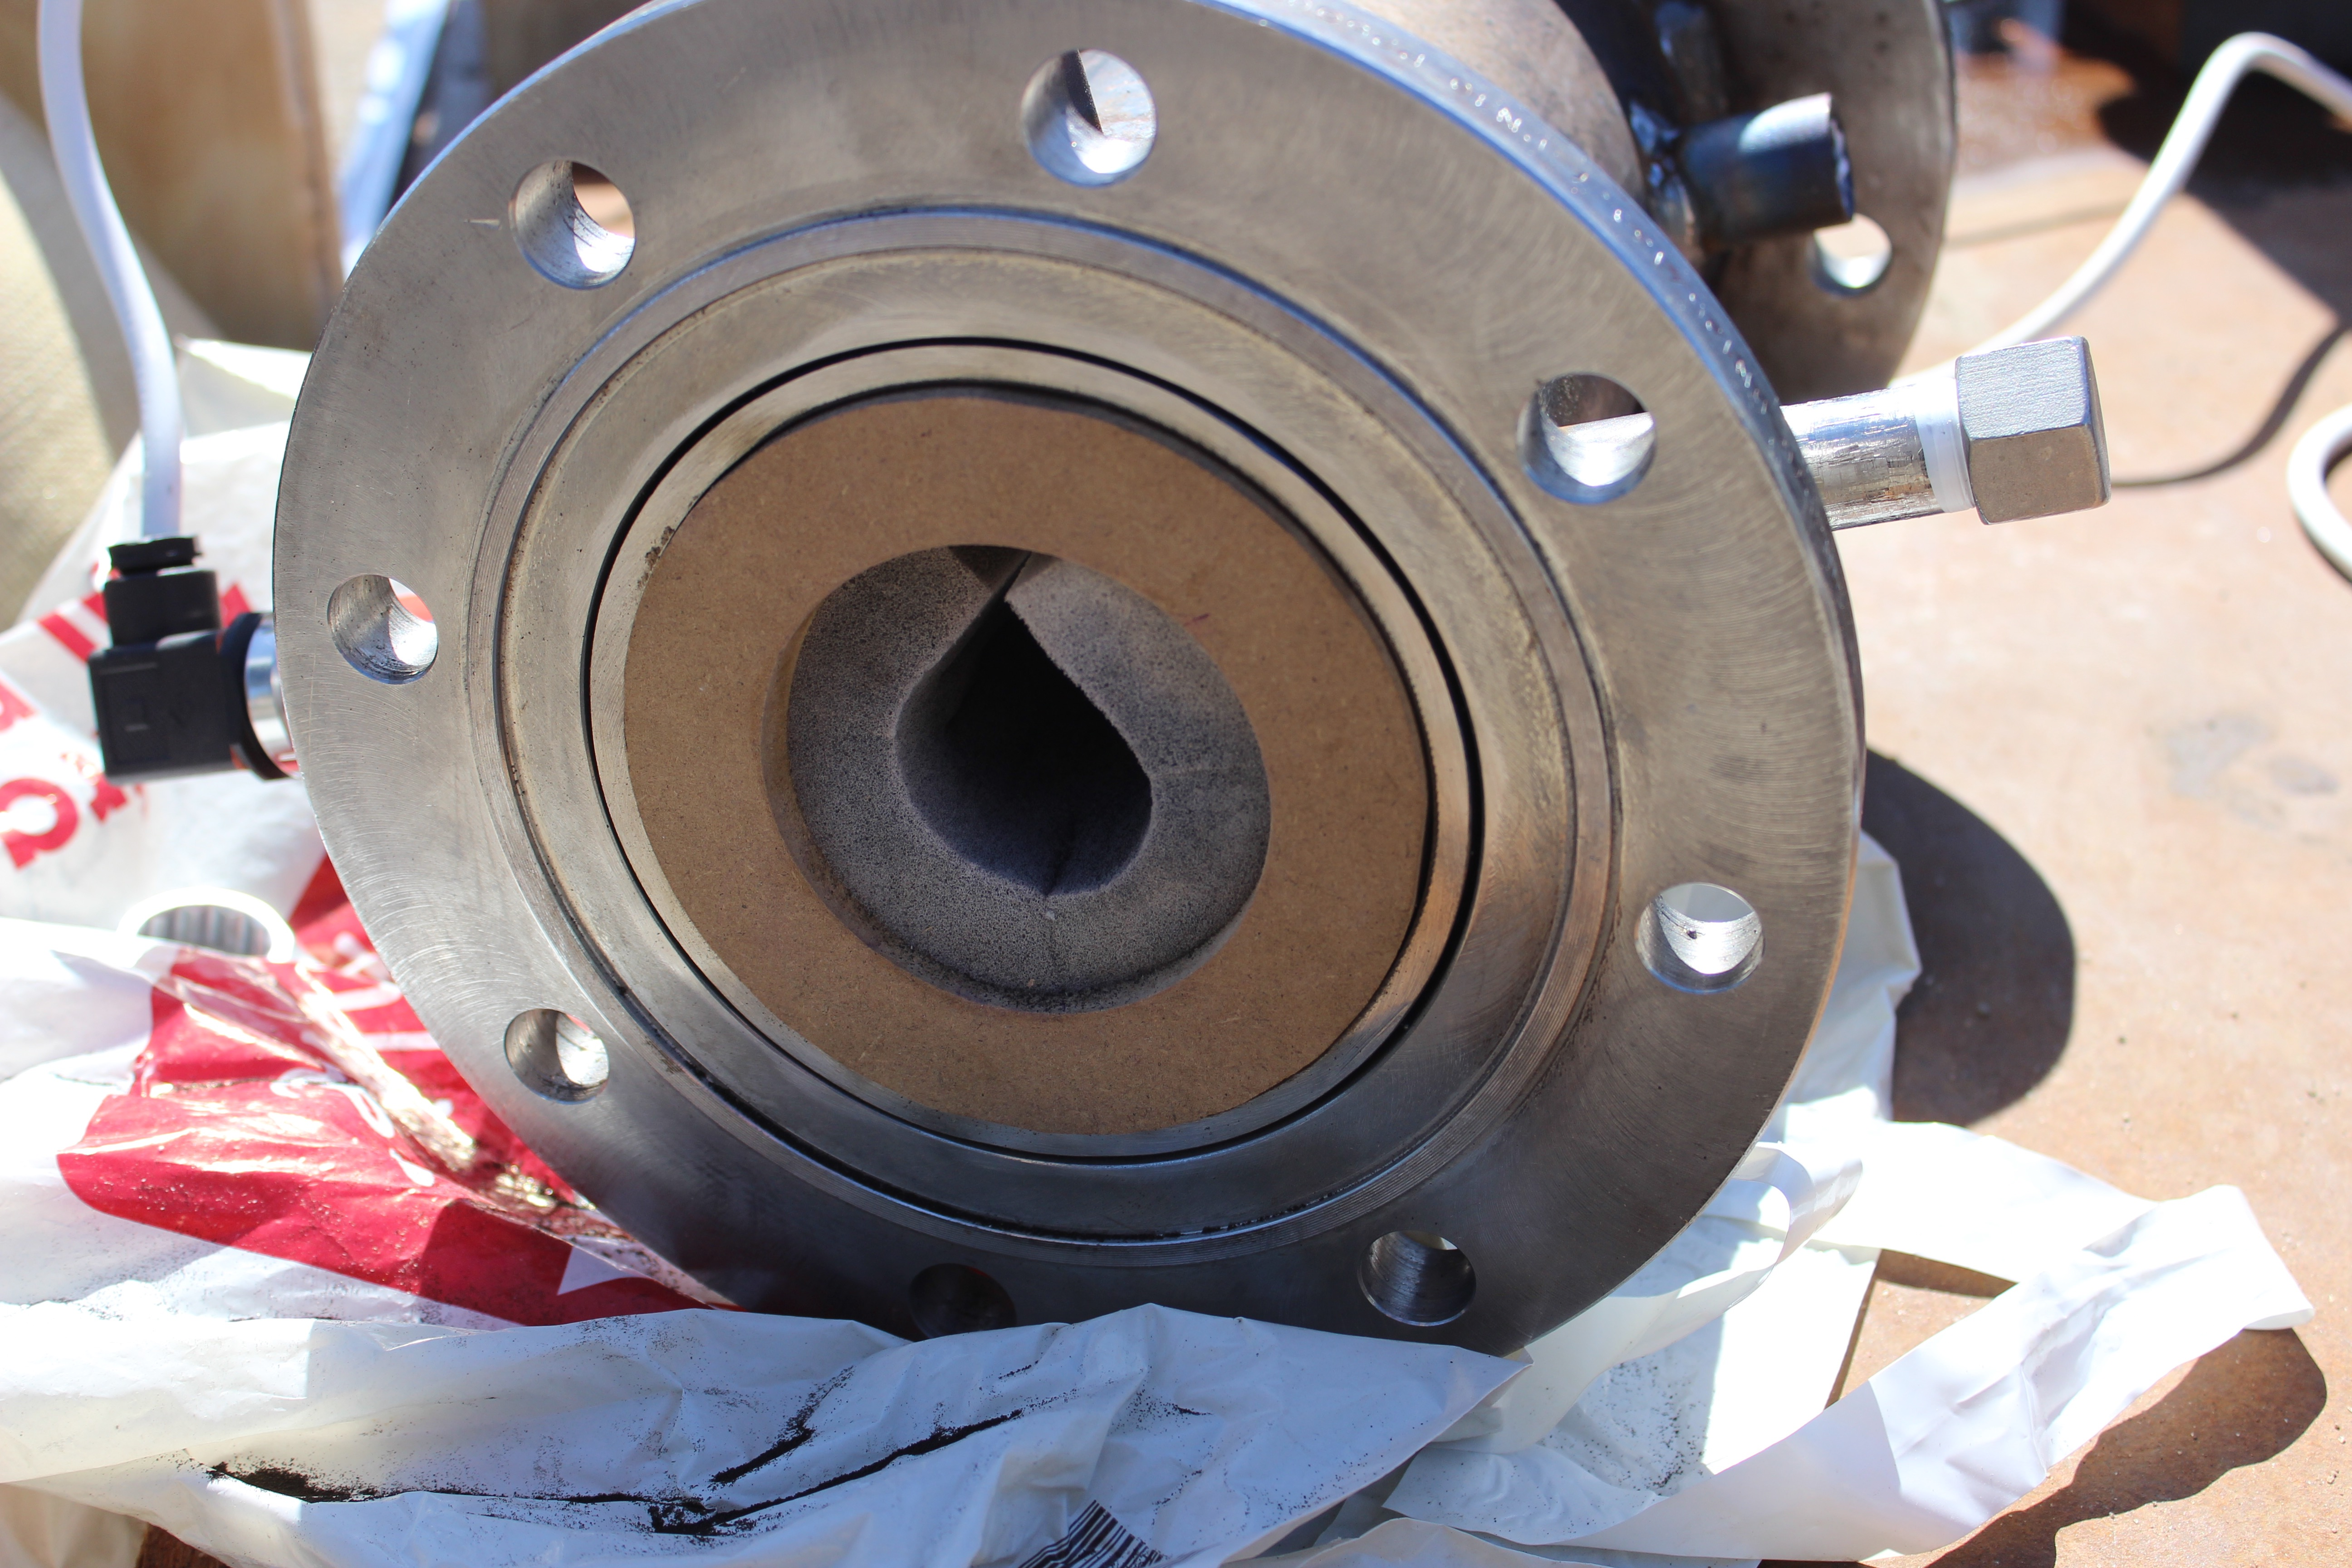
\includegraphics[width=\textwidth]{decompchamber}
		\caption{Foam permeated with \chem{KMnO_4} dust inserted into the decomposition chamber, inside a tube of MDF, in order to avoid accumulation of liquid \chem{H_2 O_2}}
		\label{fig:kmno4foam2}
	\end{figure}

	MEOWTH II was built specifically with the intent of being fast to rearm. The large flanges allows quick unbolting, and the hydrogen--peroxide tank has a quick-fill valve. The only swappable objects which changes the combustion rate is the decomposition nozzle and the fuel--grain. The tank's pressurization changed throughout the experiments, which greatly influences the flow--rate of hydrogen--peroxide. An analysis of the tank's pressure's influence on flow--rate has not been executed, however, that could be a subject for a future project. The wagon--wheel fuel grain design (see figure \ref{fig:wagonwheel}) was kept throughout the experiments, which makes the decomposition nozzle the only variable in the experiments.

	Apart from changing larger parts of the experimental setup, reloading proceduce requires swapping the rocket's interior. In figure \ref{fig:kmno4foam2}, the decomposition chamber is visible with its inner MDF--shell casing, filled with \chem{KMnO_4}--permeated foam. The inner casing prevents liquid puddles from not building up and causing trouble, in the form of instant vapourization into large quantities of gas.

	\begin{figure}
		\centering
		\includegraphics[width=\textwidth]{wagonwheelburnt}
		\caption{Wagon-wheel shaped grain as seen in figure \ref{fig:wagonwheel} after a test. Notice the wagon-wheel pattern has been burnt through, and instead a "flower"--pattern is present. Experimentally this can be seen as a small drop in pressure as seen in the results.}
		\label{fig:burntgrain}
	\end{figure}

	Swapping the wagon-wheel grain with an identical copy after every test is essential to receive consistent results, as it is worn greatly during combustion. As seen in figure \ref{fig:burntgrain}, the grain's inner walls are burnt through about two--thirds through every test. This greatly influences the grain's regression--rate, making new-- and old--grain experiments vastly different.

	Preliminary tests were done with water, as to check the newly made decomposition nozzle. Testing with water also showed leaks, making it easier to tighten and seal the piping before loading the toxic high--concentration hydrogen--peroxide. After preliminary tests, four tests were concluded and will be discussed below.

	\section{Results}
	
	All tests used $\SI{1.3}{\liter}$ of hydrogen--peroxide, making the injection rate easy to calculate assuming linear flow.	In figure \ref{fig:burnresults} the resulting pressure over time graphs are seen. As seen in the figure, higher tank pressure appears to influence the spike's height. It is questionable whether or not the spike in test three and four are representative, as data on the top appears "flattened", as if the pressure went further than the set measurement range for a brief amount of time. After the spike, the graphs flatten out and slowly decrease until they all drop slightly in pressure. This drop is most likely due to the grain's design. The wagon-wheel design seen in figure \ref{fig:wagonwheel} has a large surface area for combustion. After burning for some time the grain's wall regress far enough to create a larger cavity, but drop in overall surface area as the walls collapses to a flower--pattern as seen in figure \ref{fig:burntgrain}. As the walls are burnt through, the surface area decreases and in turn, so does the regression--rate and combustion rate. This reduces the chamber pressure by approximately $20\%$. 
	
	As the rocket is ignited noise starts to arise. This gives a clear indicator of when rocket ignition happens, but at the cost of accuracy. The noise was an unwanted feature, which stems from an accidental ground-loop in the test--setup. The rocket burns are all zeroed around the noise which shows when ignition starts after opening the ball--valve. 
	
	The first test shows a significantly slower ignition than the three others, which is most likely due to the flanges not being tightened correctly, leaking gas out the sides. Test 2 and 3 have almost identical ignition timing, although their tank--pressures differ by $\SI{7}{\bar}$. Their injectors are identical, which makes the change in spike size and timing dependent on the mass flow. It also appears that test 2 and 3 have a duration difference of almost 1 second, which is given only by the change in pressure. 
	The final test have identical tank--pressure to test 3, but with an injector with higher flow--rate. The size of the spikes are seemingly identical, however, upon further inspection it appears that the peaks are flattened due to a too low sample--range. Thus, the peak heights are not exactly representative. Interestingly, the time before ignition happens is shorter with the higher flow--rate injector. It is also quite visible that test 4 concludes much faster than the rest, after only approximately 4 seconds from initial injection, compared to the usual 6 to 8 seconds.

	\begin{figure}
		\centering
		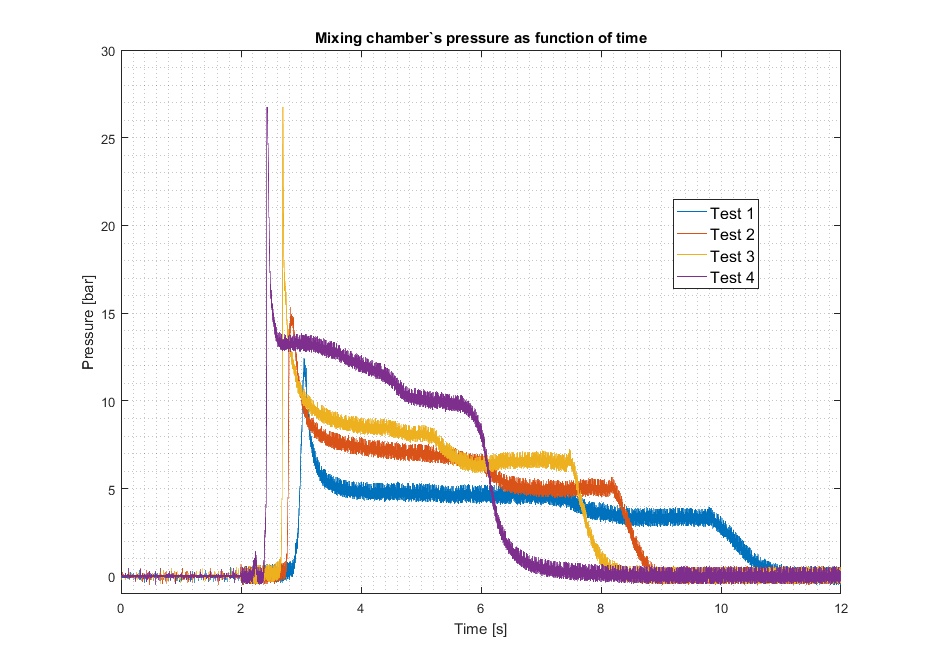
\includegraphics[width=\textwidth]{burnresults}
		\caption{Results from the four tests. Test one through four was done with pressures of $\SI{24}{\bar}, \SI{24}{\bar}, \SI{31}{\bar}$ and $\SI{31}{\bar}$ respectively. The last test was done with a larger injector.}
	\label{fig:burnresults}
	\end{figure}


% Testing of the rocket engine ensued at "Raketmadsens Rumlaboratorium" in Copenhagen on the 3rd to the 4th of may 2016. The tests were carried out by me in company by my advisor Gorm Bruun Andresen, and seven other students from Navitas.
%

%

%
% \section{Results}
%
% A total of ten measurements were collected at every test. The most essential is the Piezoelectric pressure sensors located at the front. The simulation calculates the pressure after the combustion chamber, and at the nozzle's exit.
%
% \begin{figure}
% 	\centering
% 	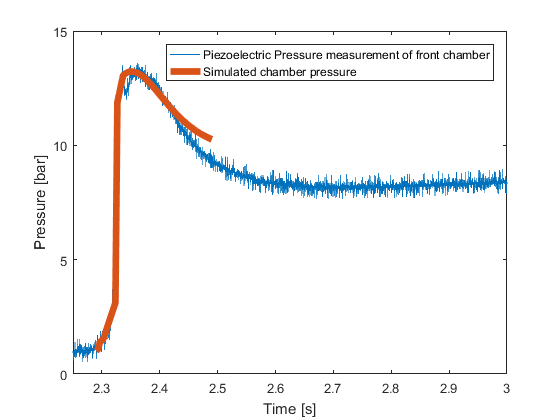
\includegraphics[width=\textwidth]{peakBurn2wsim}
% 	\caption{The second burn's front chamber peak, as found by the Piezoelectric pressure sensor. Plotted on top is the simulation created in this bachelor's thesis.}
% 	\label{fig:peakBurn2wsim}
% \end{figure}
%
% The experimental and simulation results are seen in figure \ref{fig:peakBurn2wsim}, where the blue line is the experimental results, and the red is the simulated pressure. The simulation assumes no combustion until a temperature of $\SI{220}{\celsius}$, at which all of the oxygen inside the combustion chamber is instantly consumed, followed by a steady burning phase. The instantaneous combustion looks like an explosion, as more oxygen is available at this point than at any other. The experimental front pressure dips shortly after initial combustion, which may be due to a shockwave moving through the rocket, forcing new oxygen from flowing to the grain's surface for a short period of time. The pressure then drops rapidly to a steady state, where the simulation ends just prior. The abrupt ending is due to a bug in the current version of the simulation software EES, which crashes after a certain number of iterations. Future versions may allow the calculation of the steady state. Take note of the simulation's timescale, as the duration of the peak is very small, almost only two tenths of a second.
%
%
% \begin{figure}
% 	\centering
% 	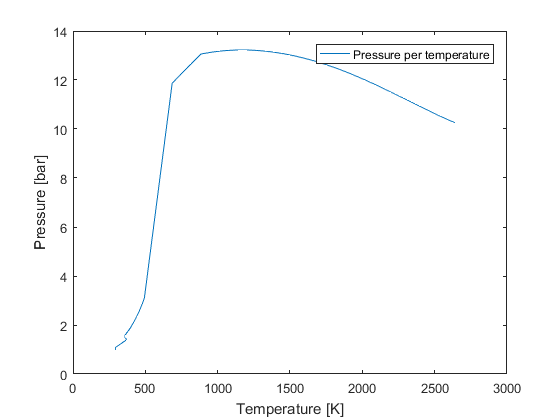
\includegraphics[width=\textwidth]{PperTsimonly}
% 	\caption{Pressure per temperature plotted over the simulated timespan in figure \ref{fig:peakBurn2wsim}. As the temperature rises, the pressure falls.}
% 	\label{fig:pressurepertemp}
% \end{figure}

% !TEX root = main.tex
\chapter{Conclusion}

From my simulation, I propose the hypothesis that the time it takes for the fuel and oxidizer to reach autoignition temperatures is the culprit of the pressure spikes observed at ignition. The proposed hypothesis is that the lower the autoignition temperature, the lower the pressure spike. Therefore, adding a preburner fuel such as ethanol or something with a low autoignition point should reduce this spike greatly. A pilotflame might be the solution to this problem as well, as piloted ignition occurs at lower temperatures, expending the available oxygen faster. Pilotflames are however quite difficult to get inside the rocket's chamber, and thus other solutions are proposed.

A proposed test experiment could be to add silane (\chem{H_4 Si}), white phosphorous (\chem{P}) or carbon disulfide (\chem{CS_2}), all which have very low (\SIlist{21;34;90}{\celsius}) autoignition points. These may work suitably as a self-igniting pilot flame, until the MDF's autoignition point is reached.
Alternatively, an "anti--test" can check the hypothesis: Increase the grain's autoignition temperature, in order to see how it behaves in the opposite limit. By increasing the autoignition temperature, a higher pressure--spike should be observed. Furthermore, pre--heating the grain to \emph{just} below its autoignition temperature using electrical heating would allow almost instant combustion as soon as oxygen reaches the heated surface. This could quite easily be tested, which makes it a possible project for the next iteration of Team Rocket.


% !TEX root = main.tex
\appendix
\chapter{Additional figures} \label{App:A}
\lipsum[1]


\chapter{News articles}\label{App:B}
Peter Madsen's blogpost on Ingeniøren:\\ \url{https://ing.dk/blog/katalytisk-aktivt-besoeg-183974}\\
P4's interview of Alex Nørgaard:\\ \url{https://drive.google.com/file/d/0B0FJw8vW3gGmY2J5SDVlcE4zaFU/view}\\
AU Engineering news' article:\\ \url{http://ingenioer.au.dk/aktuelt/nyheder/nyhed/artikel/studerende-vil-sende-raket-ud-i-rummet/}


%%%%% BIBLIOGRAPHY %%%%%
\nocite{*}
\bibliographystyle{unsrt}
\bibliography{references}
\end{document}
